\section{Konzept}

\subsection{SystemArchitektur}

Mit diesem Projekt wird Praxisruf um die Funktionen Text To Speech und Gegensprechanalge erweitert.
Um dies zu ermöglichen, sind Erweiterungen an der Systemarchitektur nötig.
Bestehende Module bleiben.
Modularität wird erweitert.
Bisher nur Package Trennung.
Neu werden Gradle Module pro Domain gemacht.
Immernoch in einem Service nachher.
Aber eine Stufe näher daran, es in Microservices aufzutrennen.
Übersichtlicher, einfacher erweitertbar.
Trennung der Domänen garantiert.

\begin{figure}[h]
    \centering
    \begin{minipage}[b]{0.9\textwidth}
        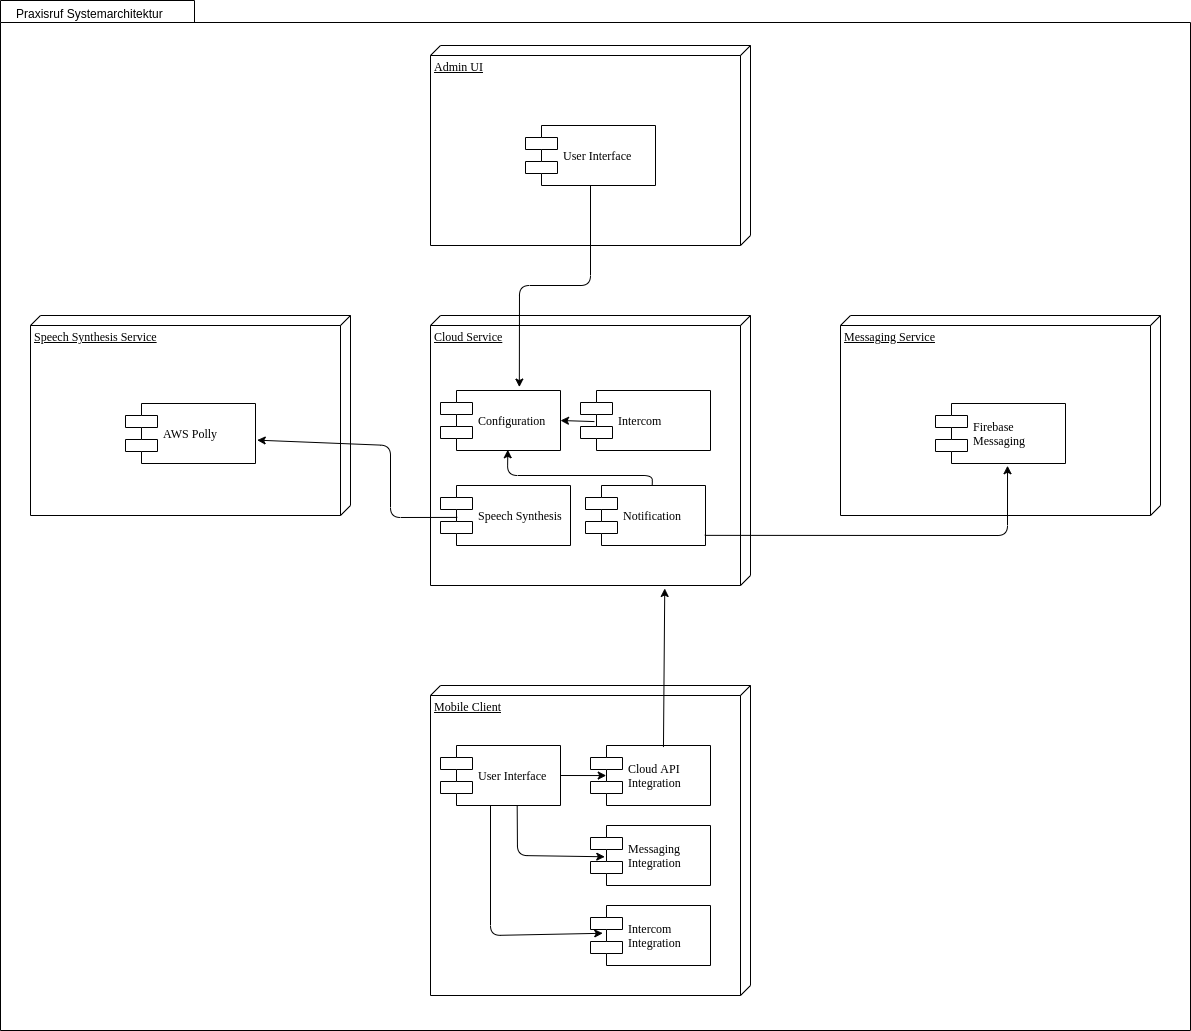
\includegraphics[width=\textwidth]{graphics/diagramms/Component_System_V01}
        \caption{Systemarchitektur Praxisruf}
    \end{minipage}
\end{figure}

\subsubsection*{Cloudservice}

Auf Seite Cloud Service werden die Module Intercom und Speech Synthesis hinzugefügt.
Intercom übernimmt das Signaling für WebRTC.
Hat den Vorteil, dass künftig auch Web und Android Clients an denselben Signaling Service angebunden werden können.
Vermittlung passiert anhand der vom Admin erfassten Konfiguration. \\

Speech Synthesis dient als einheitliche Schnittstelle zu einem externen Seepch Synthesis Service.
Dadurch kann auch wenn ein Android oder Web Client kommt, dieser genau gleich angebunden werden.
Garantie, dass die Konfiguration und Funktionsweise dieselbe für alle Clients ist. \\

\subsubsection*{Mobile Client}

Neu als nativer Client mit SwiftUI.
Beinhaltet des Benutzer Interface.
Sowie Komponenten zur Anbindung an Configuration, Notification, Speech Synthesis und Intercom.
Details in Client Kapitel. \\

\subsubsection*{Admin UI}
Das Admin UI dient weiterhin zur Administaration der Configuration.
Das Admin UI wird um Konfigurationsmöglichkeiten für Speech Synthesis und Gegensprechanalge werweitert. \\


\subsubsection*{Speech Synthesis Service}
Als neuer externer Service AWS Polly angebunden.
Dabei handelt es sich um die Speech Synthesis Funktion von Amazon Webservices. \\


\subsubsection*{Messaging Service}
Der Messaging Service wird weiterhin zum Versenden von Benachrichtigungen verwendet.
Am Messaging Service werden in diesem Projekt keine Änderungen vorgenommen. \\

\clearpage


\subsection{Migration Benachrichtigungen}

Mit IP5 wurde bereits ein Client umgesetzt.
Dieser muss für IP6 migiert werden.
Hier wird beschrieben, wie die bestehenden Anforderungen mit dem nativen client umgesetzt werden können.

\subsubsection*{Benutzeroberfläche}
SwiftUI bietet alles was man braucht.


\subsubsection*{Anbindung Cloud Service}
Anbindung an REST Schnittstellen ist mit SwiftUI natürlich Möglich.
Ein zentraler API Service wird erstellt.
Pro Domain die angesprochen wird, wird eine Extension erstellt.
Der Api Service macht den Rest call, setzt authentication.
Es muss für jeden Api Call ein Callback mitgegeben werden, dass bei completion ausgeführt wird.
Dabei muss dieses Callback den Erfolgs und den Fehlerfall behandeln. \\

Integration in die Benutzeroberfläche funktionert über einen zwischengeschalteten Service (ViewModel?).
Dieses verwendet @ObservableObject um die View über den SwiftUI Lifecycle zu aktualisieren. \\

Sämtliche Calls und Abläufe können mit diesen Mitteln analog zu IP5 umgesetzt werden.


\subsubsection*{Anbindung Firebase}

Die Anbindung von Firebase ist nicht rein mit SwiftUI möglich.
Wir benötigen die Lifecycle Integration zu iOS, die mit den AppDelegates von UIKit möglich ist.
Auch mit SwiftUI können AppDelegates verwendet werden.
Die Anbindung an Firebase Messaging wird dementsprechend mit AppDelegates gelöst.
Die Anbindung erfolgt damit wie in der offiziellen Dokumentation vorgesehen.
Damit die Abhängigkeit zu AppDelegates minimiert ist, sollen innerhalb der AppDelegates nur minimale Logik ausgeführt werden.
Die echte Logik wird an unabhängige Services delegiert.


\subsubsection*{Scheduled Reminder für Inbox}
IOS Development unterstützt scheduled tasks.

\clearpage



\subsection{Integration Text To Speech}

\subsubsection*{Benutzeroberfläche}

Erweiterung Inbox um T2S Icon. \\
Erweiterung Admin UI um Checkbox. \\
Zusätzlich Configuration Page mit preferences. \\

\subsubsection*{Konfiguration}
Erweiterung NotificationType um ein boolean Flag für isTextToSpeech.
Wenn Aktiviert, wird Benachrichtigung bei Empfang vorgelesen.
Text To Speech kann auf Client Seite dekativiert werden.
Ist es deaktiviert, werden keine Benachrichtigungen vorgelesen.
Audio Signal, dass Benachrichtung empfangen wurde ertönt aber trotzdem.
Keine zusätzlichen Endpoints am Cloud Service nötig. \\


\subsection*{Laufzeitsicht}

Empfang und Versenden gleich wie bei IP5.
Benachrichtigung enthält zudem neu Flag ob T2S gebraucht werden soll.
Wenn ja, wird Vorlesen an T2S Service delegiert.

\begin{figure}[h]
    \centering
    \begin{minipage}[b]{0.9\textwidth}
        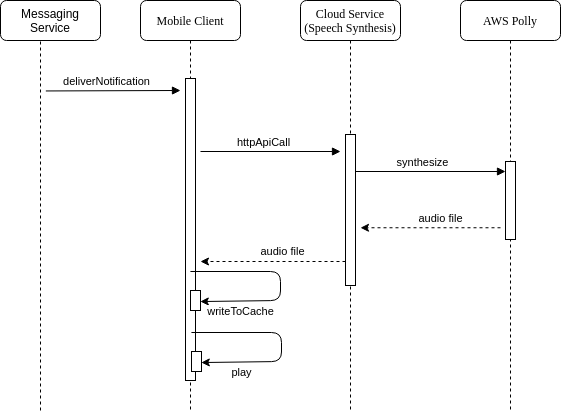
\includegraphics[width=\textwidth]{graphics/diagramms/Sequence_Speech_Synth_V01}
        \caption{Ablauf Benachrichtigung empfangen}
    \end{minipage}
\end{figure}

\clearpage

\subsection{Integration Gegensprechanlage}

\subsubsection*{Benutzeroberfläche}

Button Screen wie IP5 \\
Active Call Screen \\
Erweiterte Inbox \\
Neue Screens für Gegensprechanlage. \\
Erweiterung Admin UI für Konfiguration CallType \\


\subsubsection*{Konfiguration}
Erweiterung Configuration Domain um CallType.
Hat text property, dass als Anzeige auf dem Button dient.
Hat Liste von Clients, die im Call angesprochen werden können.

\subsubsection*{Laufzeitsicht}

\begin{figure}[h]
    \centering
    \begin{minipage}[b]{0.9\textwidth}
        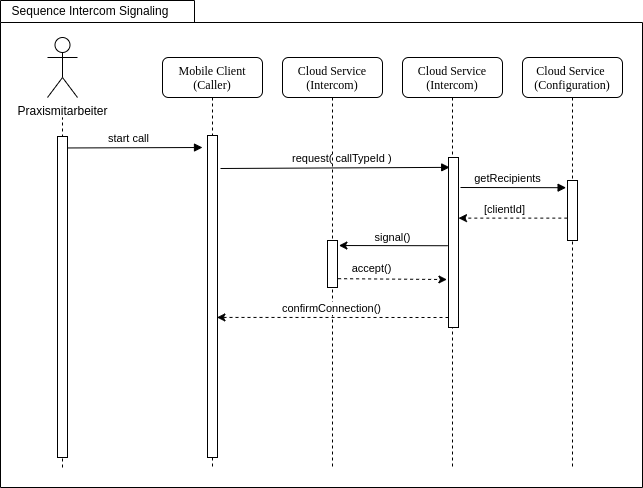
\includegraphics[width=\textwidth]{graphics/diagramms/Sequence_Intercom_Broking_V01}
        \caption{Ablauf Verbindungsaufbau Gegensprechanalge}
    \end{minipage}
\end{figure}

\clearpage

\subsection{Übersicht Erweiterung Praxisruf Cloud Service}

<< Erweitertes ERD für Configuration Domain (Cloud Service) >>

\clearpage
